%-------------------------------------------------------------------
% bachelor thesis - presentation
%
% topic: ACDC4JS - How to analyze a JavaScript garbage collector
%
% create by: Mario Preishuber
% create date: 2014, Jan 01.
%-------------------------------------------------------------------
\section{Experiments}

%\begin{frame}
%	\frametitle{Content}
%	\setcounter{tocdepth}{2}
%	\tableofcontents[currentsection]
%\end{frame}

\begin{frame}
	\frametitle{Experiments}
	\begin{itemize}
		\item Step 1: Simple but artificial mutator
		\item Step 2: Obtaining a realistic heap model
		\item Step 3: Developing a realistic JavaScript mutator (TODO)
	\end{itemize}
\end{frame}

\newcounter{StepCounter}
\stepcounter{StepCounter}

\subsection{Step \theStepCounter: Simple but artificial mutator}
\begin{frame}
	\frametitle{Step \theStepCounter: Simple but artificial mutator}
	\begin{itemize}
		\item Get information about the garbage collector
		\begin{itemize}
			\item Collection frequency %cycle
			\item Quantity of collected memory
			\item Number of collected objects
		%	\item type of garbage collection
		\end{itemize}
		
		\smallskip
		\pause
			
		\item Prepare a simple mutator
		\begin{itemize}
			\item Number of allocated objects
			\item Number of live objects
			\item Size of an object
		\end{itemize}
			
		\smallskip
		\pause
			
		\item Wrap system measurements
		\begin{itemize}
			\item Execution time
			\item Real memory (resident set size ... rss) 
		\end{itemize}
	\end{itemize}
\end{frame}
\begin{frame} 
	\frametitle{Step \theStepCounter: Measurements - allocation only}
	\begin{center}
		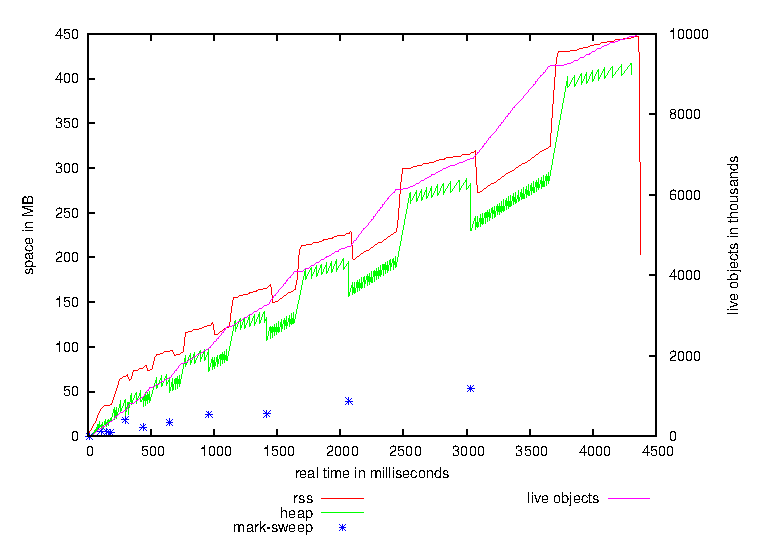
\includegraphics[width=.9\textwidth]{keep_all_obj_rss_heap_mas_obj_time}
	\end{center}
\end{frame}
\begin{frame} 
	\frametitle{Step \theStepCounter: Measurements - execution time}
	\begin{center}
		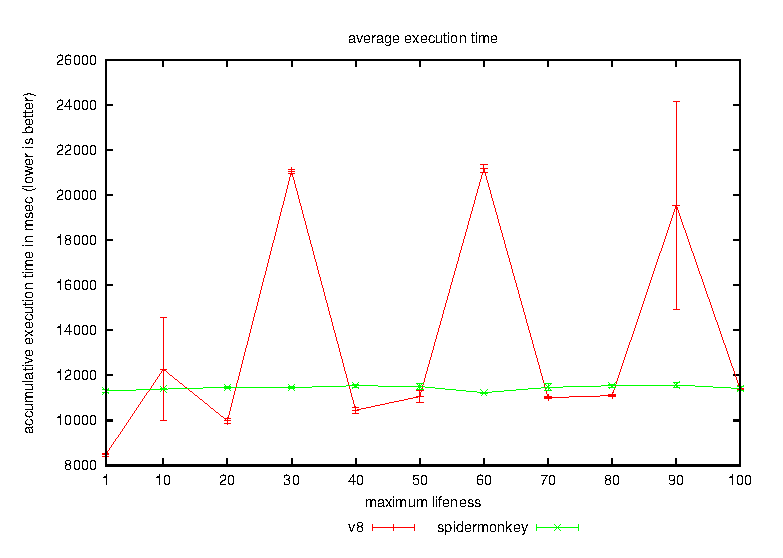
\includegraphics[width=.9\textwidth]{acdc_multi_exec_time}
	\end{center}
\end{frame}
	
\stepcounter{StepCounter}
\subsection{Step \theStepCounter: Obtaining a realistic heap model}
\begin{frame}
	\frametitle{Step \theStepCounter: Obtaining a realistic heap model}
	\begin{itemize}
		\item Important for mutator implementation
		\item Customizations
		\begin{itemize}
			\item Custom Chromium binary
			\item Custom V8 binary
		\end{itemize}
			
		\pause
			
		\item Tools for JavaScript heap analysis
		\begin{itemize}
			\item AutomatedUserInteraction
			\item HeapSnapshotAnalyzer
		\end{itemize}
	\end{itemize}
\end{frame}
	
\begin{frame}
	\frametitle{Step \theStepCounter: Obtaining a realistic heap model}		
	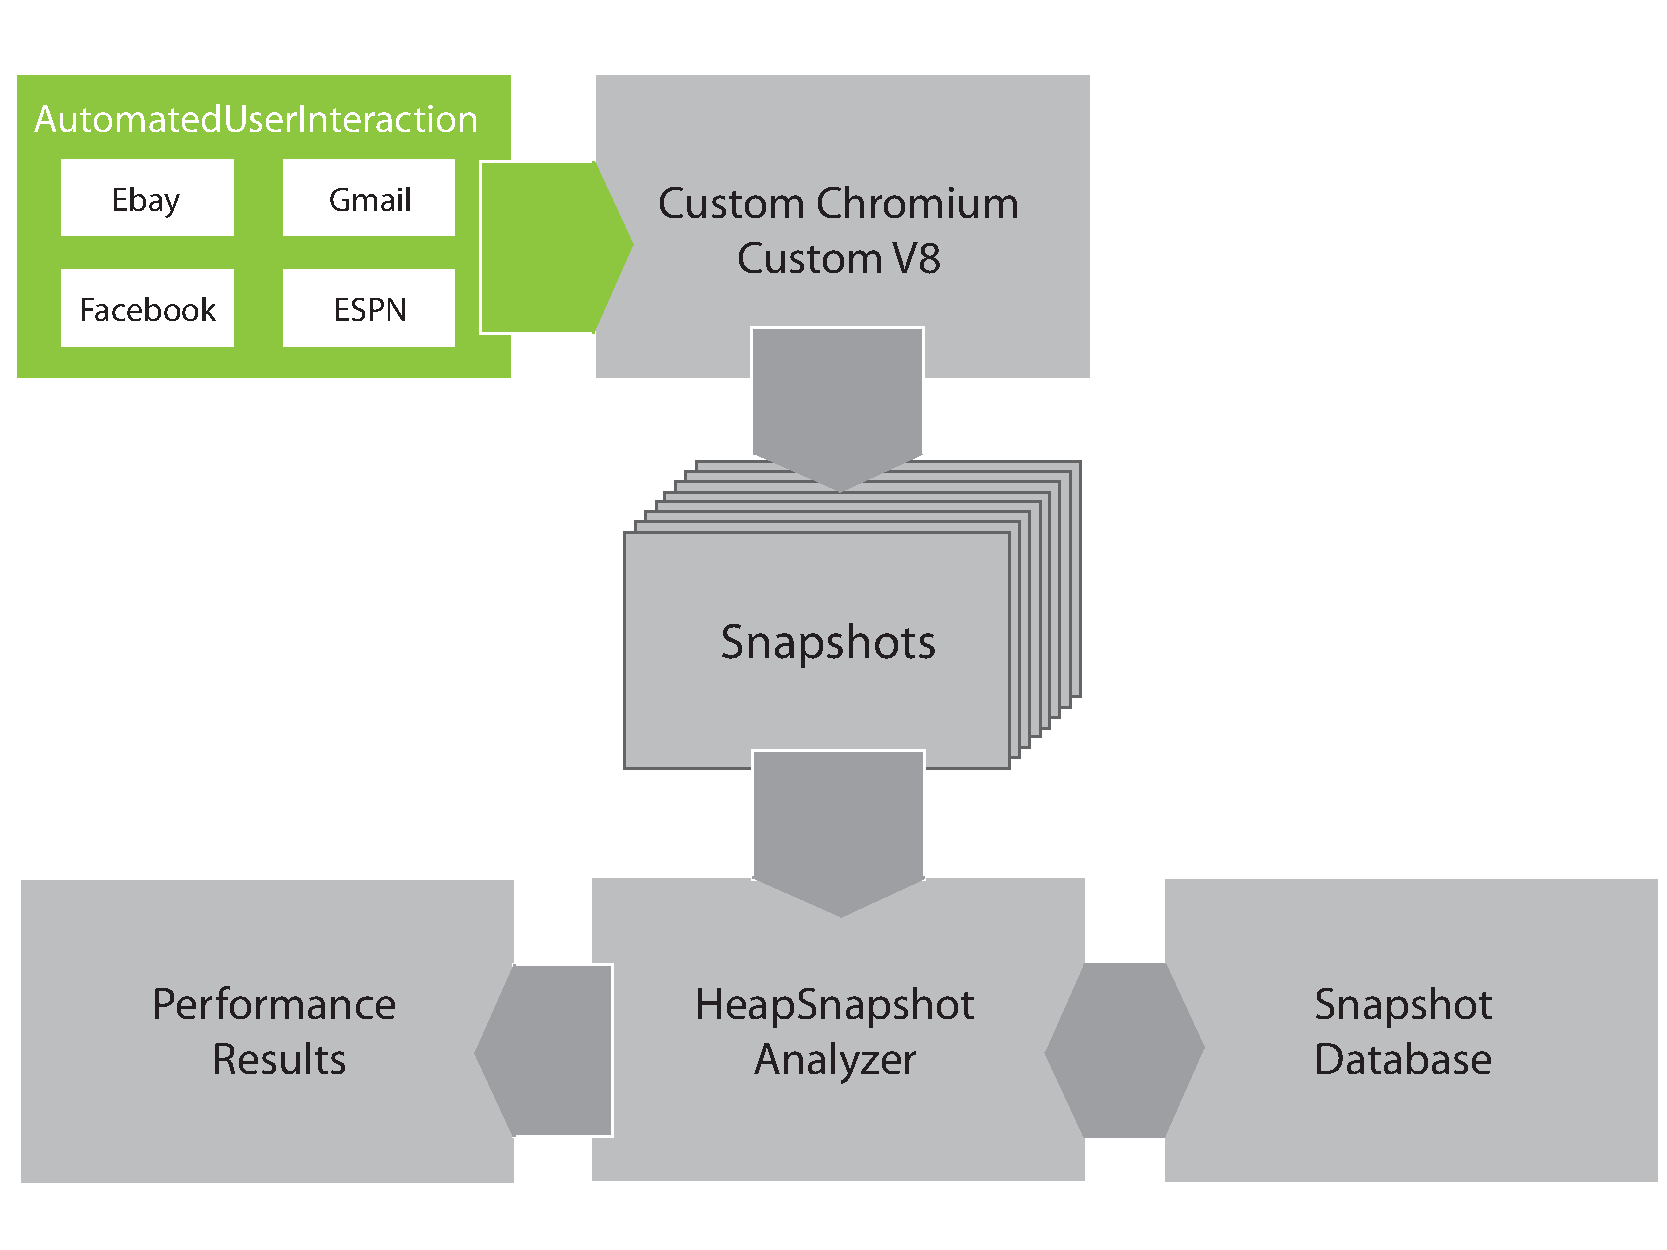
\includegraphics[width=26em]{solution_h_1}
\end{frame}

\subsubsection{AutomatedUserInteraction}
\begin{frame}
	\frametitle{AutomatedUserInteraction}
	\begin{itemize}
		\item Java application
		\item SeleniumHQ framework for automated user interaction
		\begin{itemize}
			\item \href{http://www.seleniumhq.org/}{http://www.seleniumhq.org}
		\end{itemize}
		\item Web applications
		\begin{itemize}
			\item \textbf{News:} CNN, ESPN, The Economist
			\item \textbf{Email:} Gmail, Hotmail
			\item \textbf{Shops:} Ebay, Amazon
			\item \textbf{Maps:} Google, Bing
			\item \textbf{Search:} Google, Bing
			\item \textbf{Social:} Facebook, Google Plus
		\end{itemize}
	\end{itemize}
\end{frame}
	
\begin{frame}
	\frametitle{Step \theStepCounter: Obtaining a realistic heap model}		
	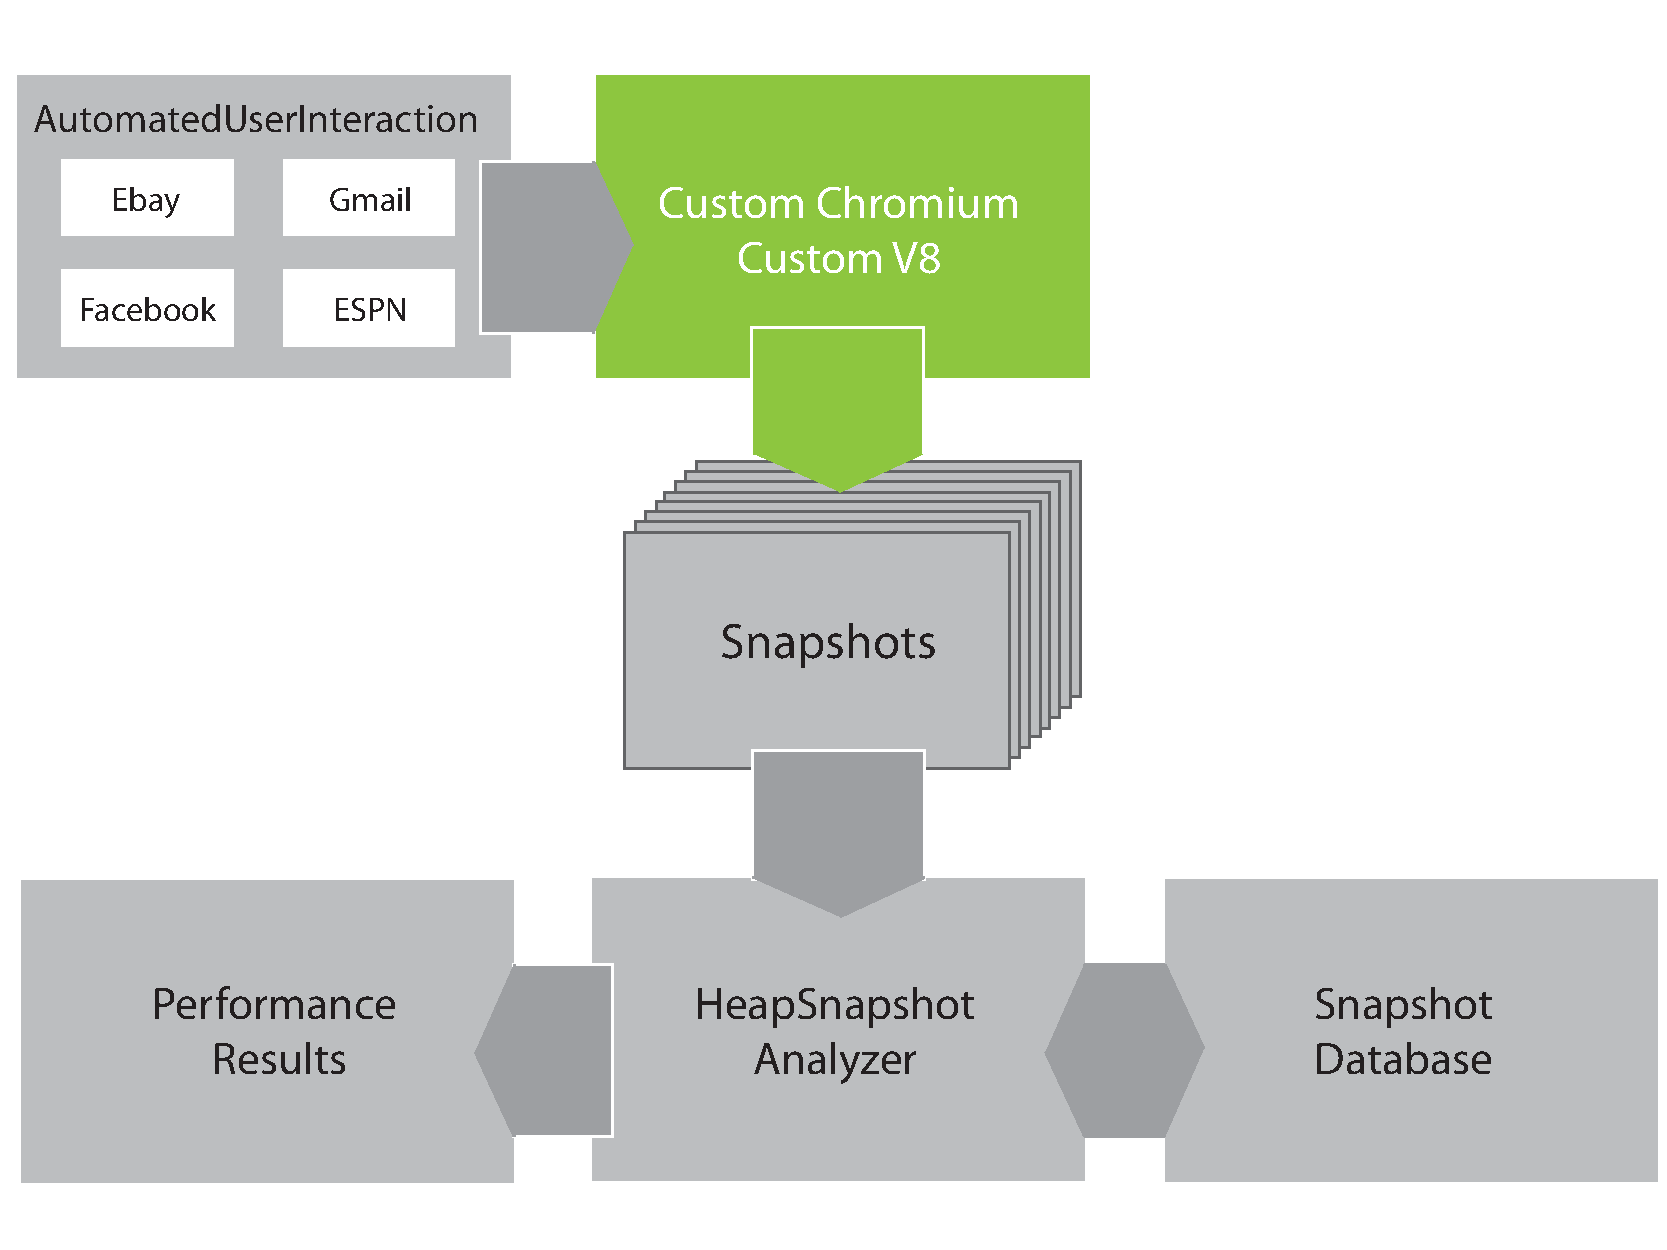
\includegraphics[width=26em]{solution_h_2}
\end{frame}

\subsubsection{Customizations}
\begin{frame}
	\frametitle{Customizations}
	%\begin{columns}
	%	\begin{column}{.55\linewidth}
	%		Custom Chromium binary
	%		\begin{itemize}
	%			\item Used flags
	%			\begin{itemize}
	%				\item \texttt{no\_sandbox} 						% Disables the sandbox for all process types that are normally sandboxed.
	%			\end{itemize}
	%		\end{itemize}
			
			Custom V8 binary
			\begin{itemize}
				\item New flags
				\begin{itemize}
					\item \texttt{automatic\_heap\_snapshots} 		% create heap snapshot automatically every heap-snapshot-interval KBs
					\item \texttt{heap\_snapshot\_interval} 		% heap snapshot interval in KB
					\item \texttt{heap\_snapshot\_prefix} 			% prefix for the .heapsnapshot files
				\end{itemize}
				\item Used flags
				\begin{itemize}
					\item \texttt{gc\_interval} 					% garbage collect after n allocations
				\end{itemize}
			\end{itemize}
	%	\end{column}
	%	\begin{column}{.35\linewidth}			
	%		\includegraphics<1>[width=9em]{chromium_v}
	%	\end{column}
	%\end{columns}
\end{frame}
	
\begin{frame}
	\frametitle{Step \theStepCounter: Obtaining a realistic heap model}		
	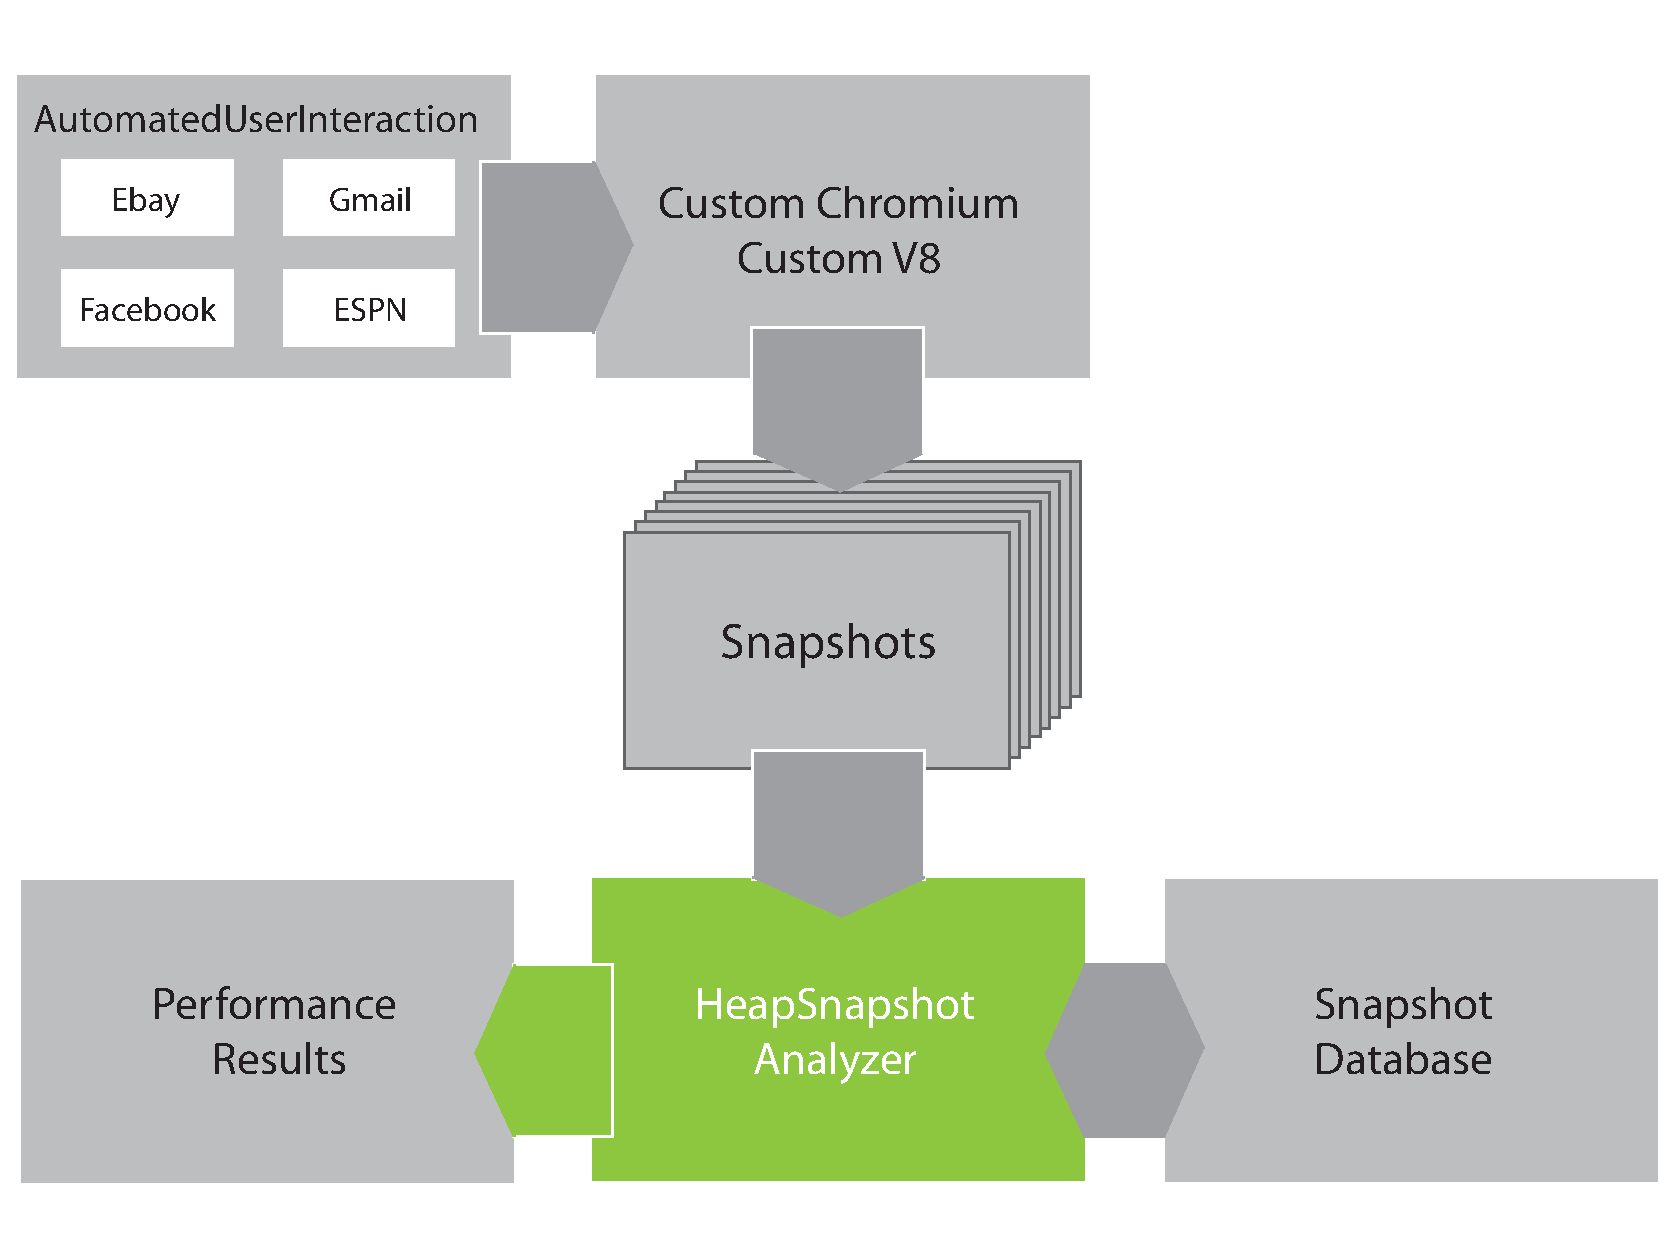
\includegraphics[width=26em]{solution_h_3}
\end{frame}
	
\subsubsection{HeapSnapshotAnalyzer}
\begin{frame}
	\frametitle{HeapSnapshotAnalyzer}
	\begin{itemize}
		\item Java application
		\item PostgreSQL 9.3
		\item Write snapshots into database
			
		\pause
			
		\item Heap graph
		\begin{itemize}
			 \item Number of leafs
			 \item Number of nodes
			 \item Number of edges
			 \item Number of strongly connected components
		\end{itemize}
			
		\pause 
			
		\item Node characteristics
		\begin{itemize} 
			 \item In-degree
			 \item Out-degree
			 \item Root distance
			 \item Node size 
		\end{itemize}
	\end{itemize} 
\end{frame}
	
%\begin{frame}
%	\frametitle{Step \theStepCounter: Obtaining a realistic heap model}		
%	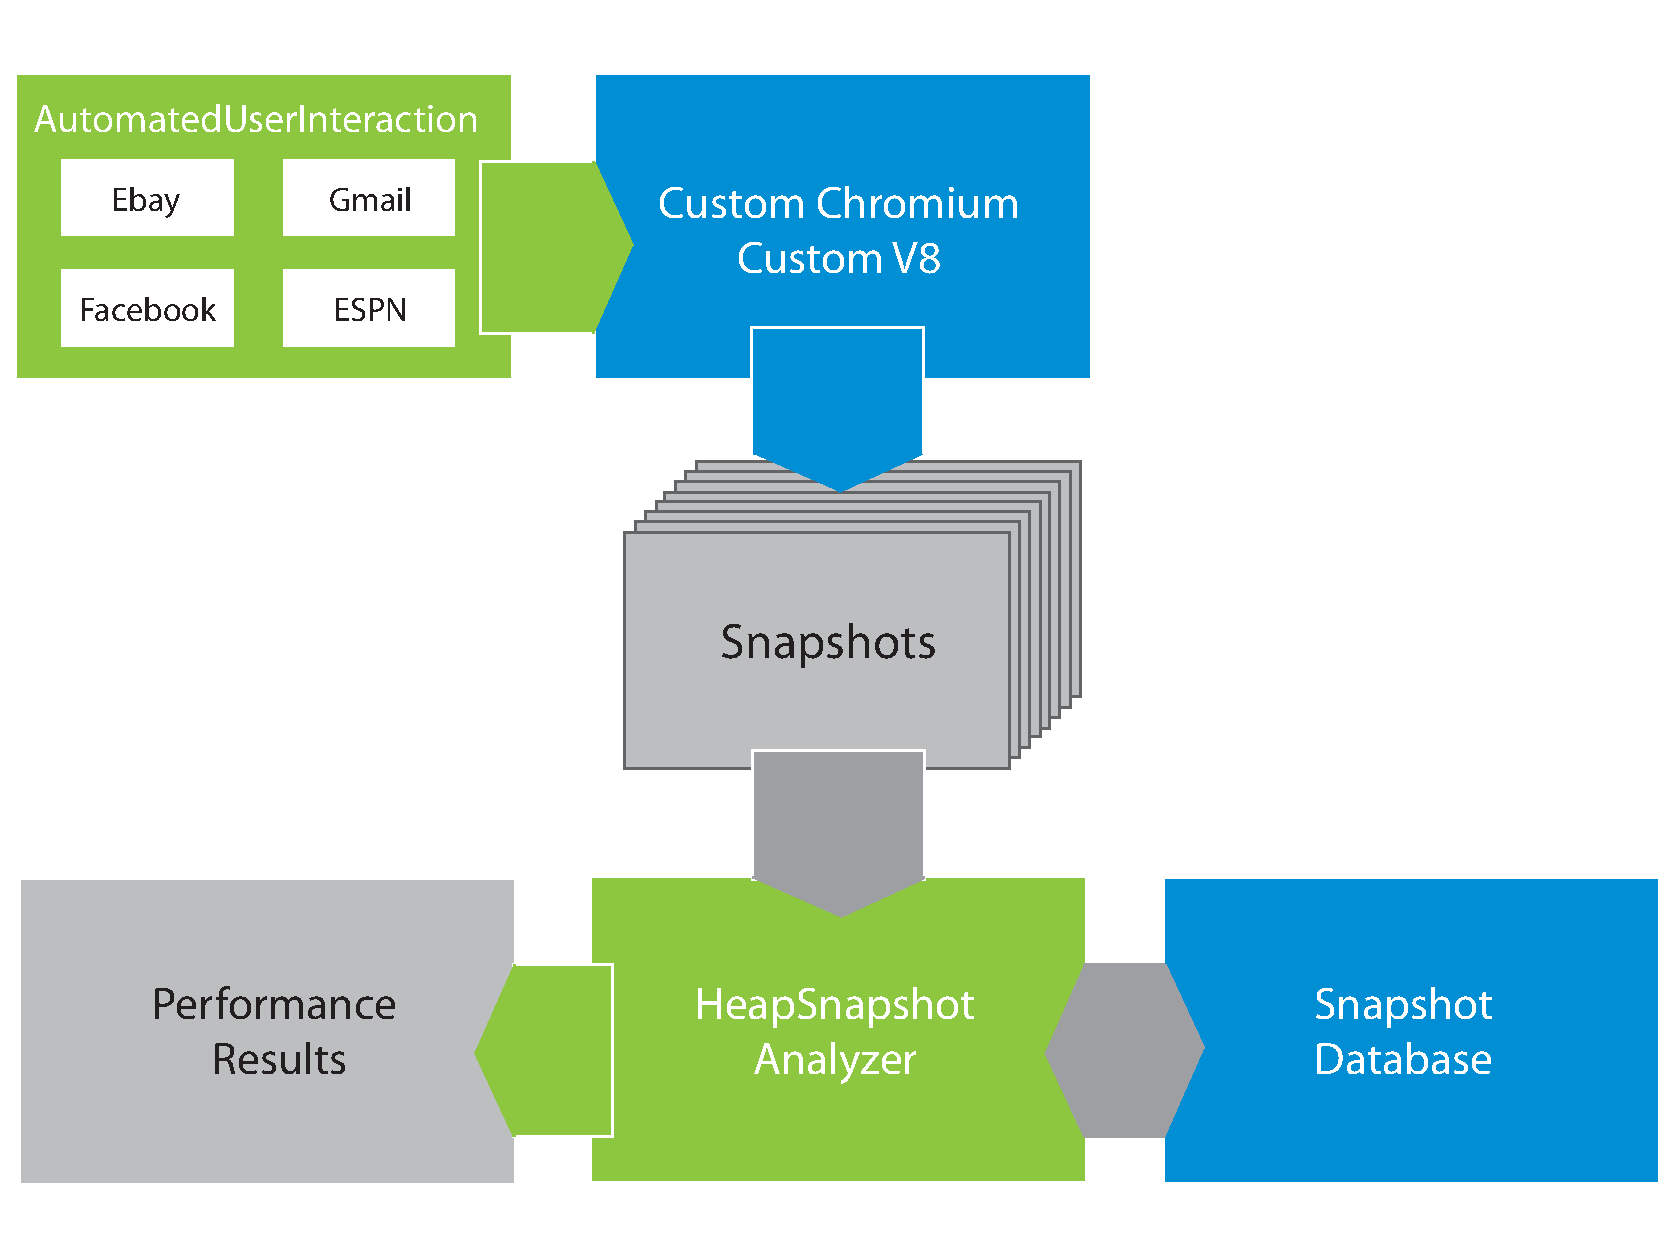
\includegraphics[width=26em]{solution_h}
%\end{frame}
	
\stepcounter{StepCounter}
\subsection{Step \theStepCounter: Developing a realistic JavaScript mutator (TODO)}
\begin{frame}
	\frametitle{Step \theStepCounter: Developing a realistic JavaScript mutator (TODO)}
	\begin{center}
		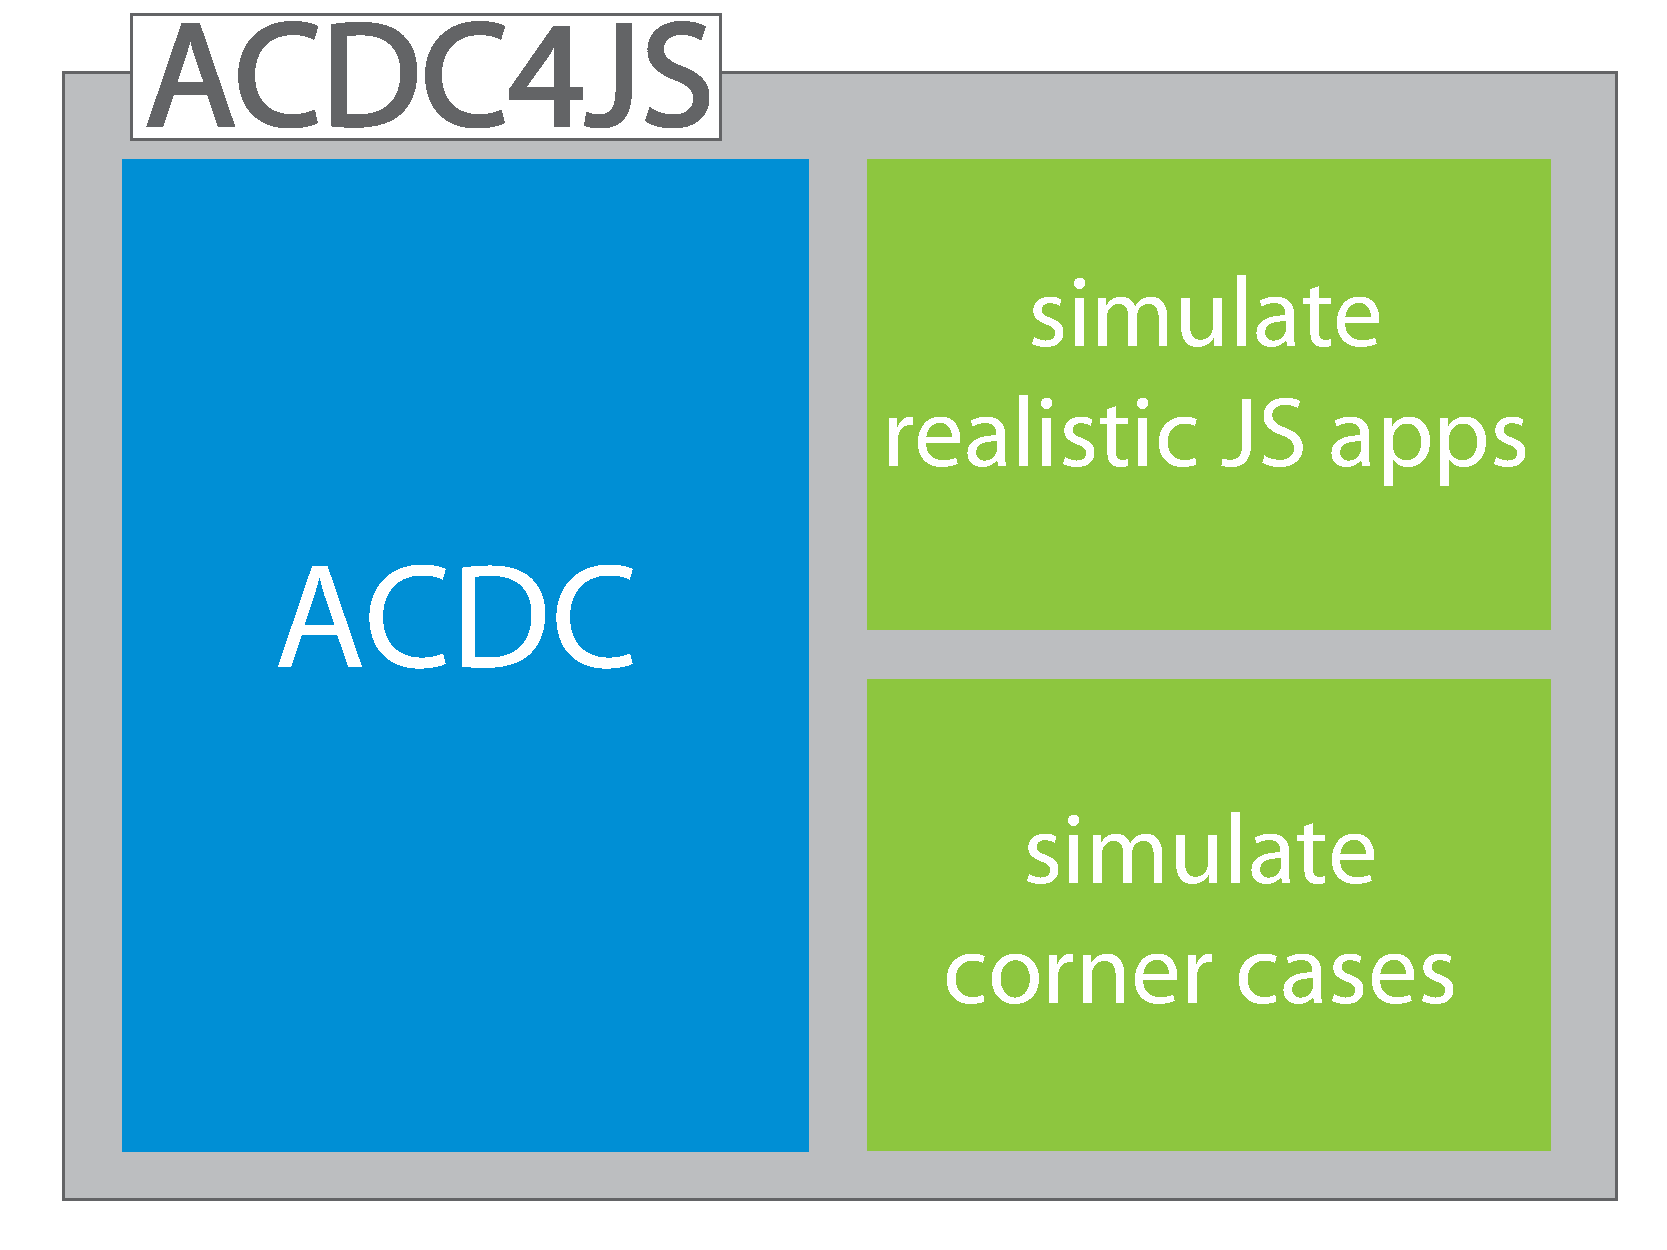
\includegraphics[width=22em]{acdc4js}
	\end{center}
\end{frame}

%		Develop a universal JavaScript mutator based on the real web application analyzation results.  
	% Develop a 
	% \begin{itemize}
	% 	\item Universal JavaScript mutator
	% 	\item Based on the original ACDC implementation
	% \end{itemize}
	% 	
	% \pause
	% 	
	% Extend this mutator
	% \begin{itemize}
	% 	\item With special features for garbage collector measurements
	% 	\item Based on the analysis results simulate
	% 	\begin{itemize}
	% 		\item real web applications and
	% 		\item corner cases 
	% 	\end{itemize}
	% \end{itemize}